\chapter{Desarrollo}

	A continuaci\'on se describe de forma detallada, el diseño y desarrollo del paquete \textbf{apnnClassifier} disponible en: \url{ https://github.com/ghouljd/apnnClassifier } para la clasificaci\'on de tub\'erculos de papa criolla(\textit{Solanum phureja}) para diferentes densidades de siembra empleando redes neuronales probabil\'isticas, siguiendo la metodolog\'ia descrita en el Cap\'itulo 3.
	
\section{Creación del esqueleto del paquete.}
	
	Para esta fase se utilizó el ambiente de desarrollo RStudio, el cual es un entorno integrado de fuente abierta para R que agrega muchas caracter\'isticas y herramientas de productividad, además de facilitar el uso de R integrando la ayuda y la documentación.\\

En esta primera etapa se creó la estructura del paquete, la cual está conformada por la identificación por nombre y descripción del paquete (Figura 4.1), además, se cargan los paquetes del CRAN de R y sus extensiones, de los cuales dependen los métodos y funciones que permitiran el desarrollo del paquete \textbf{apnnClassifier}; los mismos fueron almacenados en el repositorio local que se crea para este paquete durante el proceso de desarrollo; los principales fueron:\\

\begin{itemize}
\item pnn(Chasset, P. \textit{et. al}, 2013;\url{https://cran.r-project.org/web/packages/pnn/index.html})
\item pROC(Robin, X. \textit{et. al}, 2019; ;\url{https://cran.r-project.org/web/packages/pROC/index.html})
\item dplyr(Wickham, H. \textit{et. al}, 2019;;\url{https://cran.r-project.org/web/packages/dplyr/index.html})
\item roxygen2(Ooms, J. \textit{et. al}, 2018;;\url{ https://cran.r-project.org/web/packages/roxygen2/index.html})
\end{itemize}

\begin{figure}[h!]
	\caption{Descripción del paquete}
	\centering
	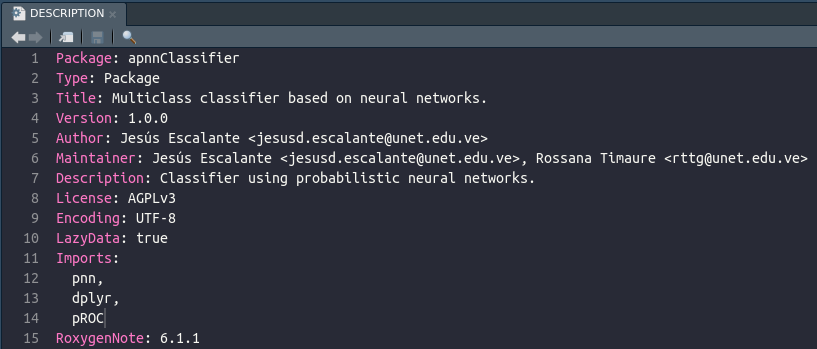
\includegraphics[scale=0.6]{package-description.png}
	\label{fig2:arch}
\end{figure}

\section{Diseño de las soluciones algorítmicas.}

\subsection{Diseño de las soluciones algorítmicas para el entrenamiento de una red neuronal probabilística que permita la clasificación de tubérculos de papa.}

	El objetivo funcional del paquete desarrollado es permitir al usuario realizar el entrenamiento de una red neuronal probabilística para la clasificación de datos estandarizados o no estandarizados, así como graficar y evaluar los resultados de la clasificación.\\

	Para este fin se desarrollaron 2 funciones, necesarias para llegar a los resultados esperados y una opcional para estandarizar los datos de entrada. \\

	Como entrada para iniciar el proceso de entrenamiento y clasificación, es necesario tener un  conjunto de datos de entrenamiento en una estructura \textit{ data.frame}, teniendo conocida cual es la columna que identifica las clases del conjunto; así como tener un conjunto de datos de entrenamiento en forma de matriz con la misma cantidad de columnas como variables clasificadoras tenga el conjunto de entrenamiento.\\

	Las funciones antes mencionadas junto a sus entradas, salidas y diagramas de flujos serán descritas a continuación.\\


\subsection{Diseño del algoritmo de la función de entrenamiento y clasificación de la red (trainNeuralNet).}

	Para el caso de la creación y entrenamiento de la red neuronal probabilística para permitir la clasificación de los datos, se diseñó el ingreso de los datos en dos conjuntos de datos, uno de entrenamiento con la columna de clase incluida y un conjunto de pruebas con la misma cantidad de datos de entrenamiento que el primer conjunto, además de, el índice de la columna indicadora de clase en el conjunto de entrenamiento y el valor óptimo de la función de activación en caso de conocerse (Cuadro \ref{tabla:entradasTrainNeuralNet}.). La función diseñada hace uso del paquete \textbf{PNN} (Chasset, P) de R para crear y entrenar una red neuronal probabilística, el algoritmo de la función se encarga de crear, entrenar, optimizar y clasificar los datos del conjunto de pruebas recibido, obteniendo al final una red neuronal entrenada capaz de clasificar y lista para ser evaluada junto a su clasificación (Figura \ref{fig:trainNeuralNet}).\\

\begin{table}[htb]
\begin{center}
\begin{tabular}{|p{3cm}|p{5cm}|p{8cm}|}
\hline
\multicolumn{3}{|c|}{\textbf{Entradas}} \\
\hline
\textbf{Nombre} & \textbf{Descripción} & \textbf{Reglas} \\
\hline \hline
train\_set & Conjunto de entrenamiento & Parámetro de tipo \textit{data.frame}. Requerido. \\ \hline
test\_set & Conjunto de pruebas & Parámetro de tipo \textit{matriz}. Requerido. \\ \hline
category\_column & Índice de la columna que identifica la categoría o clase en el conjunto de entrenamiento & Parámetro de tipo \textit{entero}. No requerido. Valor por defecto: 1. \\ \hline
sigma & Valor óptimo de la función de activación & Parámetro de tipo \textit{flotante}. No requerido. Es calculado en caso de ausencia del parámetro. \\ \hline
\end{tabular}
\caption{Entradas de la función de entrenamiento - \textbf{trainNeuralNet}.}
\label{tabla:entradasTrainNeuralNet}
\end{center}
\end{table}

\begin{figure}[h!]
	\caption{Diagrama de flujo para función de entrenamiento y clasificación de la red neuronal probabilística}
	\centering
	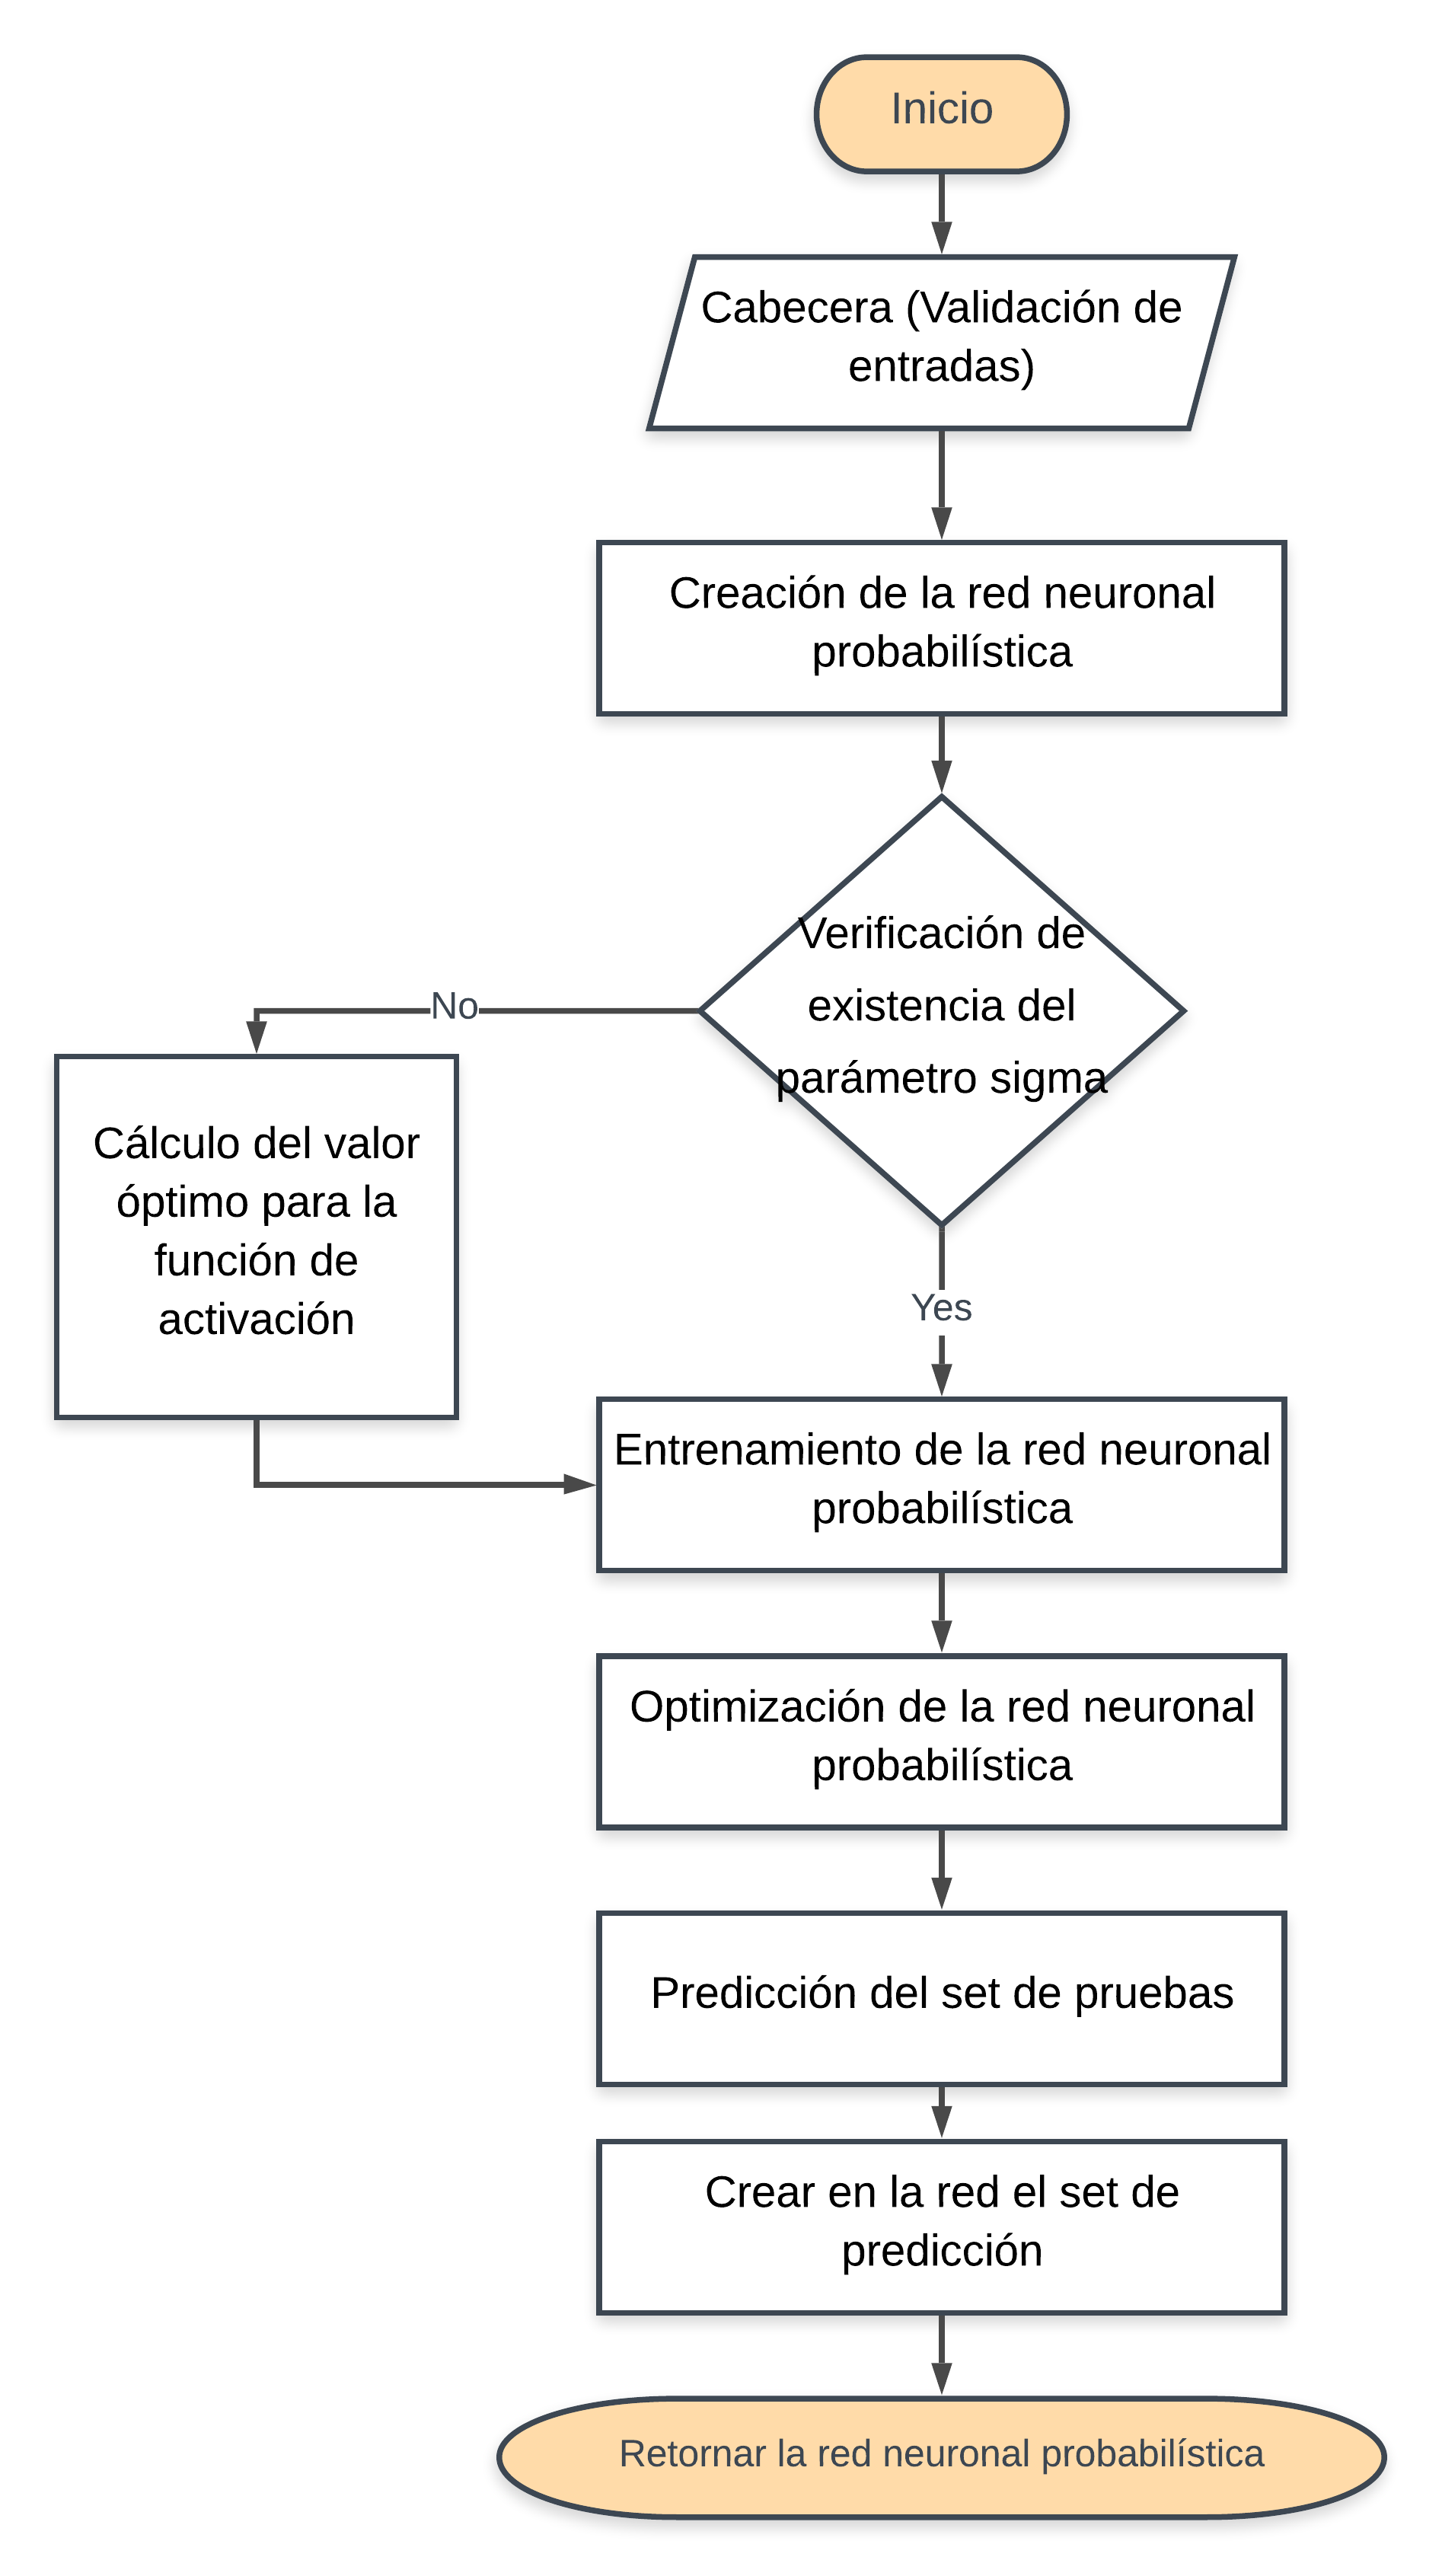
\includegraphics[scale=0.18]{trainNeuralNet.png}
	\label{fig:trainNeuralNet}
\end{figure}

\subsection{Diseño del algoritmo de la función de evaluación de la red neuronal probabilística y su clasificación (evaluate).}

	Para el caso de la evaluación de la red neuronal probabilística y su clasificación, se unificó el ingreso de los datos en la lista de R que se traduce a la red neuronal probabilística que es salida de la función \textbf{trainNeuralNet}, descrita anteriormente (Cuadro \ref{tabla:entradasEvaluate}). La función diseñada realiza la creación del gráfico de nubes de puntos, para demostrar la correlación entre las variables de entrenamiento y hace uso del paquete \textbf{pROC} (Robin, X) de R para crear el gráfico de curvas características operativas (Curvas ROC) para identificar si la clasificación fue buena, el algoritmo también permite observar datos de análisis de la red como su sensibilidad, efectividad y área bajo la curva, para determinar un mal o un buen análisis (Figura \ref{fig:evaluate}. ).\\

\begin{table}[htb]
\begin{center}
\begin{tabular}{|p{3cm}|p{5cm}|p{8cm}|}
\hline
\multicolumn{3}{|c|}{\textbf{Entradas}} \\
\hline
\textbf{Nombre} & \textbf{Descripción} & \textbf{Reglas} \\
\hline \hline
pnn & Red neuronal probabilística & Parámetro de tipo \textit{lista}, que es salida de la función descrita en la sección 4.3. Requerido. \\ \hline
\end{tabular}
\caption{Entradas de la función de evaluación - \textbf{evaluate}.}
\label{tabla:entradasEvaluate}
\end{center}
\end{table}

\begin{figure}[h!]
	\caption{Diagrama de flujo para función de evaluación de la red neuronal probabilística}
	\centering
	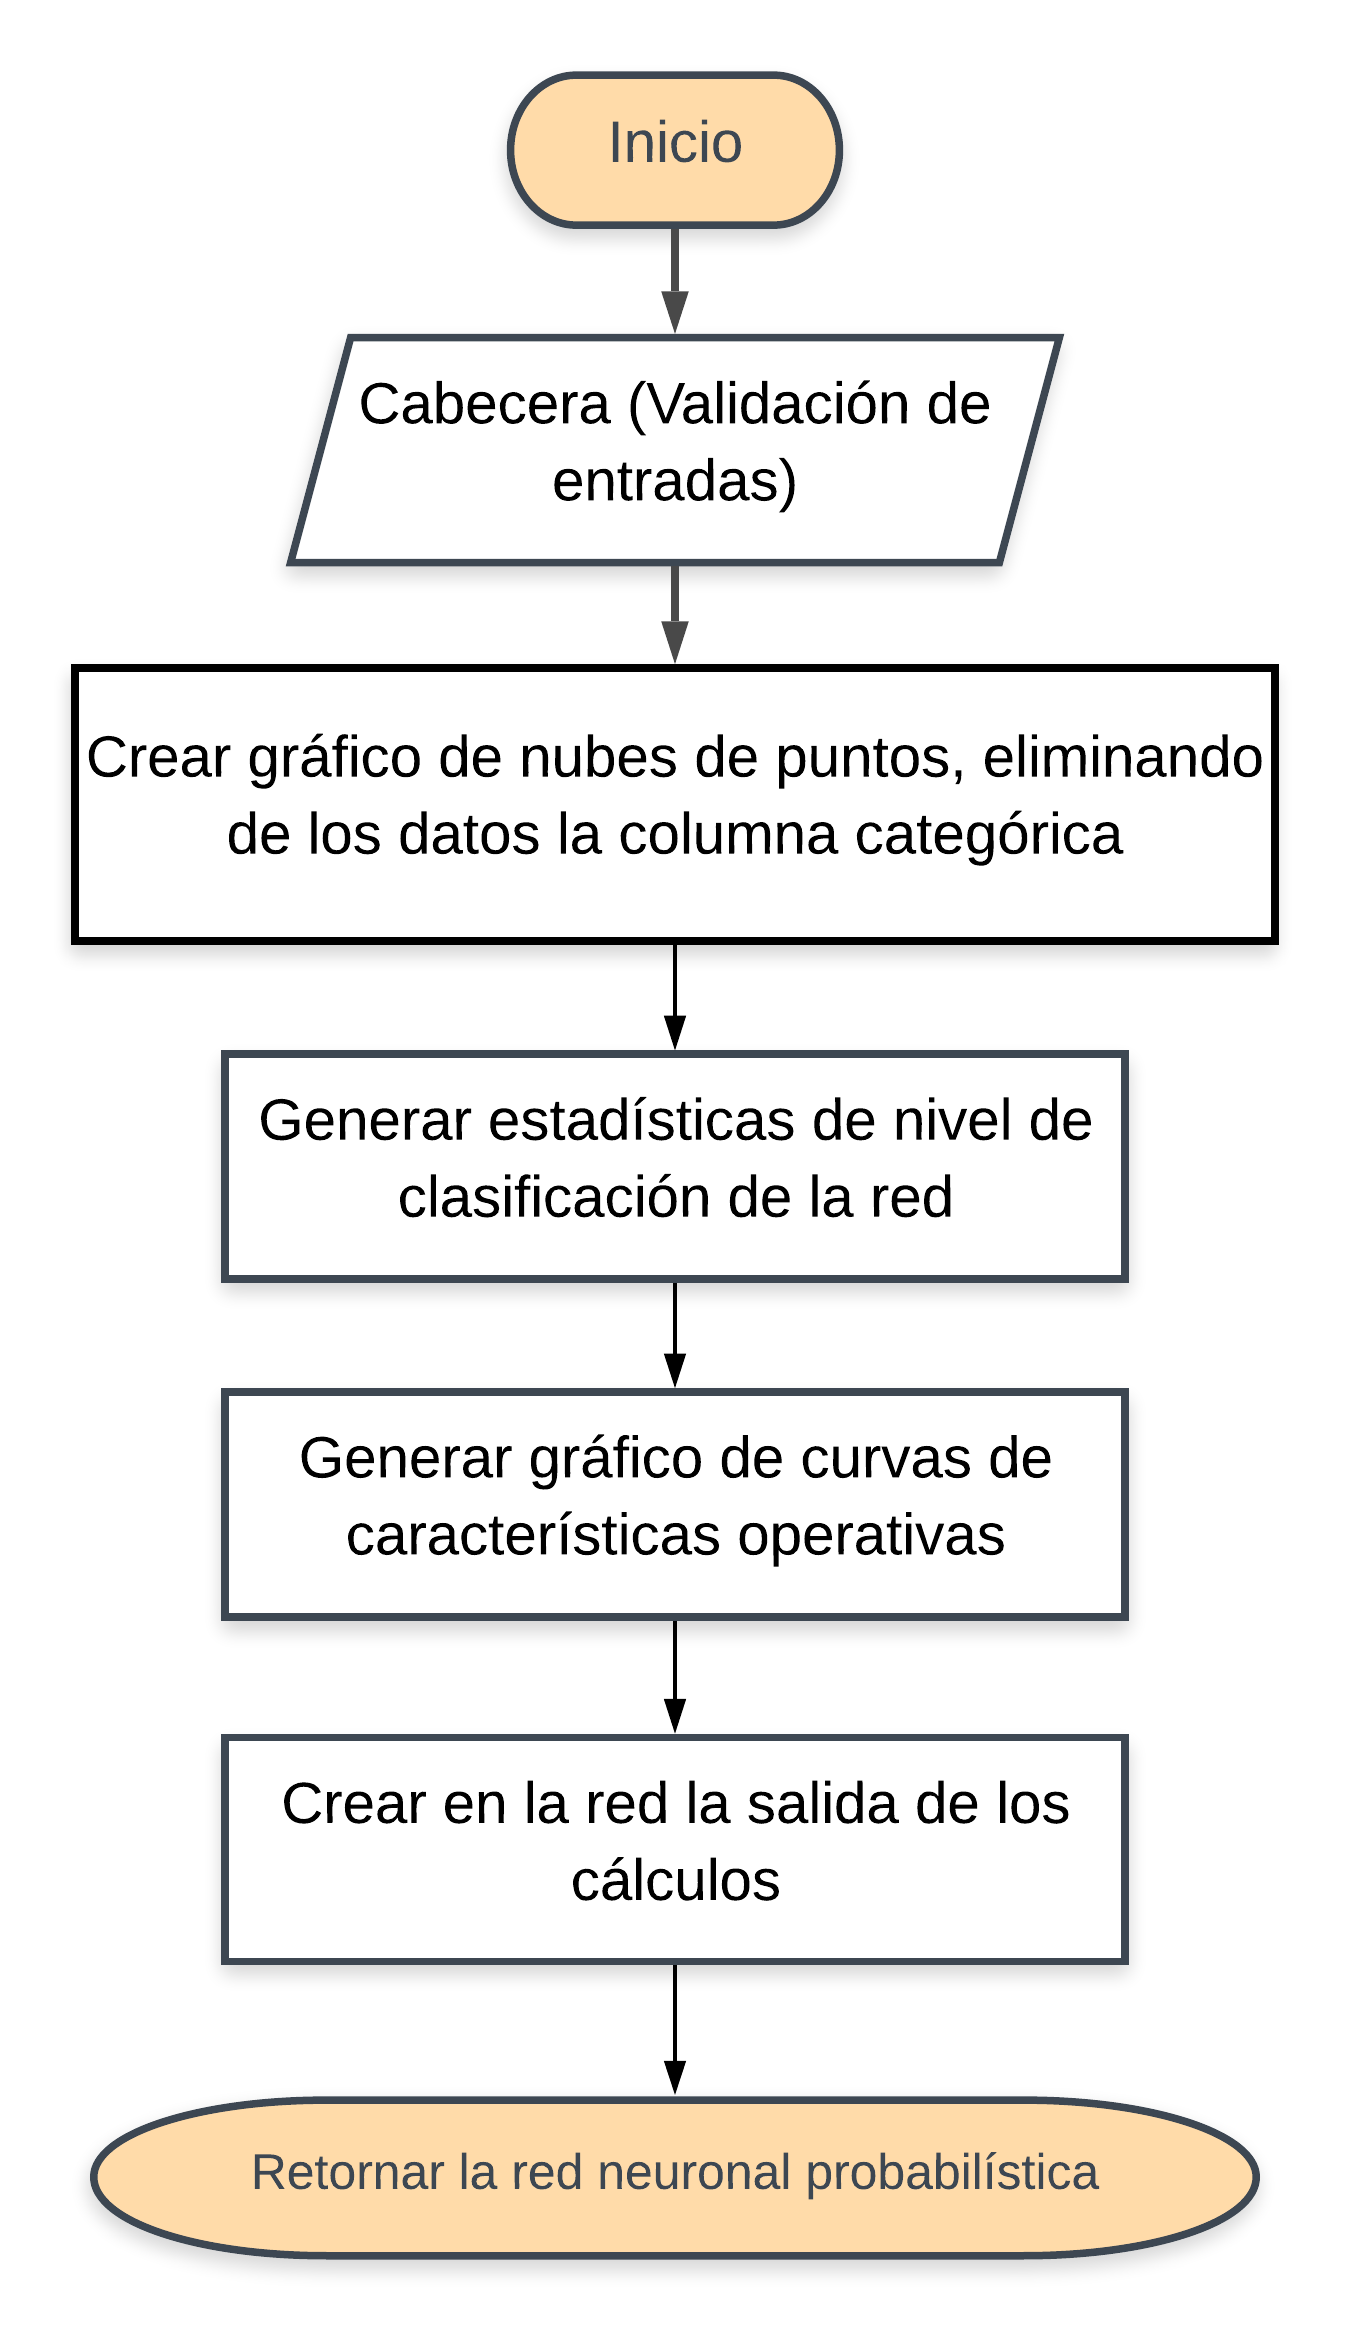
\includegraphics[scale=0.8]{evaluate.png}
	\label{fig:evaluate}
\end{figure}

	La predicción del conjunto de pruebas se puede observar en el atributo “output” de la red neuronal devuelta por la función y es un \textit{data.frame} con dos columnas, una que tiene la predicción y otra con la probabilidad con la que se obtuvo dicha predicción, como se puede observar en la figura \ref{fig:outputTesting}. \\
	
\begin{figure}[h!]
	\caption{Ejemplo de predicción de set de pruebas.}
	\centering
	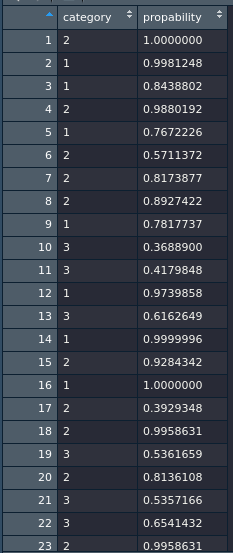
\includegraphics[scale=0.8]{outputTesting.png}
	\label{fig:outputTesting}
\end{figure}

\subsection{Diseño del algoritmo de la función de estandarización de datos (standardize).}

	Para el caso de la estandarización opcional de los datos, se diseñó el ingreso de los datos en un conjunto en formato \textit{lista} o \textit{data.frame}, para este paso se debe tener en cuenta que no tiene sentido alguno estandarizar la columna clase. El tipo de estandarización a usar, que puede ser puntual por media y varianza o escalar por minimos y máximos (Cuadro\ref{tabla:entradasStandardize}). La función diseñada dependiendo del tipo de estandarización indicado en la entrada, aplica la función de estandarización columna por columna del conjunto de datos (figura \ref{fig:standardize}).\\
	
\begin{table}[htb]
\begin{center}
\begin{tabular}{|p{3cm}|p{5cm}|p{8cm}|}
\hline
\multicolumn{3}{|c|}{\textbf{Entradas}} \\
\hline
\textbf{Nombre} & \textbf{Descripción} & \textbf{Reglas} \\
\hline \hline
set & Conjunto de datos & Parámetro de tipo \textit{lista} o \textit{data.frame}. Requerido. \\ \hline
type & Tipo de estandarización & Parámetro de tipo cadena de caracteres. No requerido. Valores posibles: "punctual" - "scale". Valor por defecto: "punctual".\\ \hline
\end{tabular}
\caption{Entradas de la función de estandarización - \textbf{evaluate}.}
\label{tabla:entradasStandardize}
\end{center}
\end{table}

\begin{figure}[h!]
	\caption{Diagrama de flujo para función de  estandarización de datos}
	\centering
	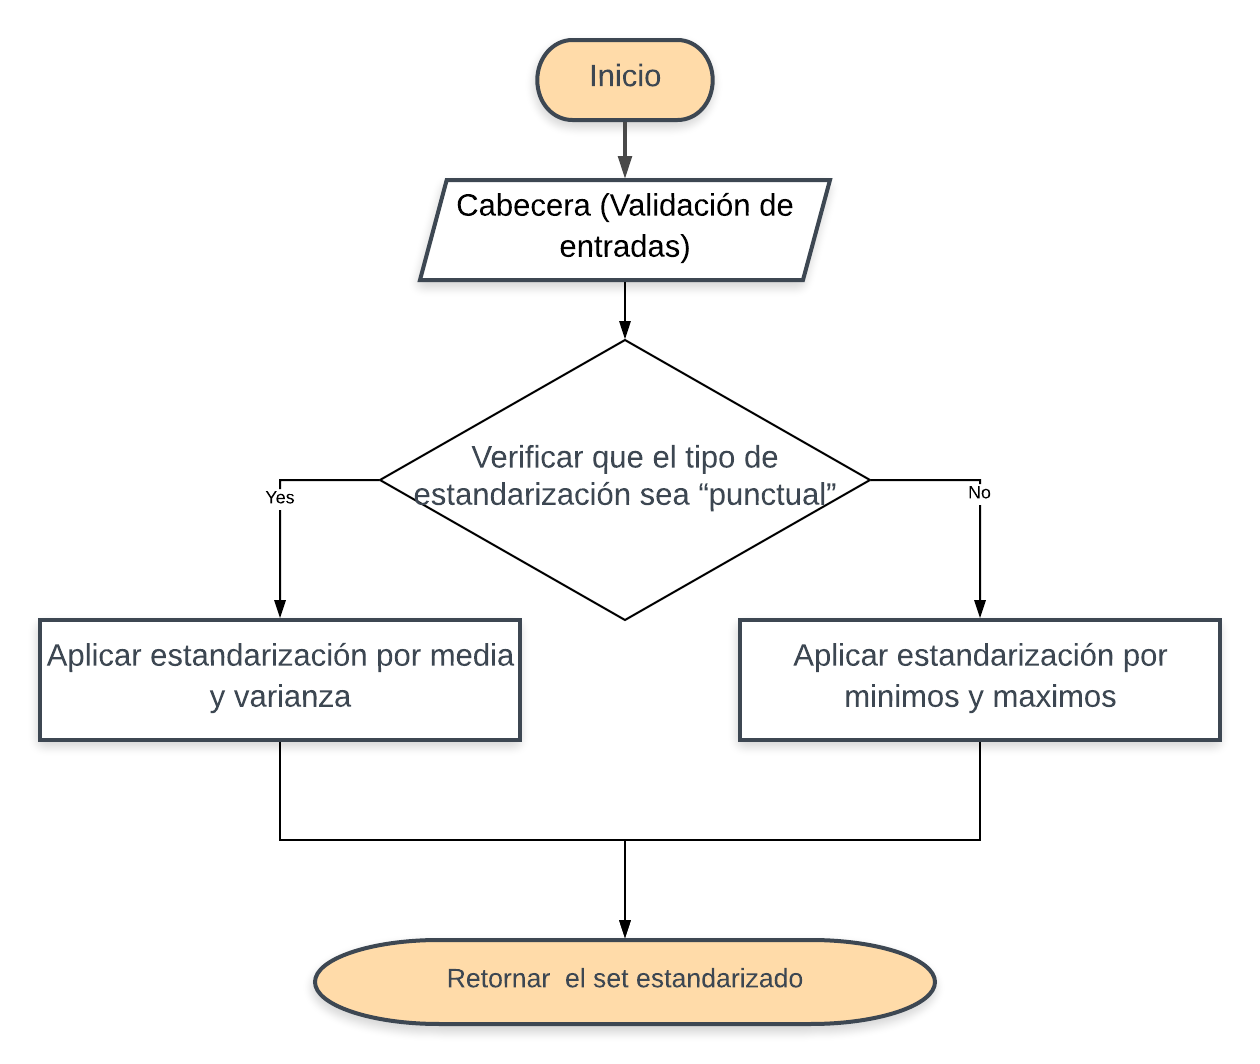
\includegraphics[scale=0.8]{standardize.png}
	\label{fig:standardize}
\end{figure}

\section{Codificación de los algoritmos}

	La codificación de los algoritmos se realizo en el IDE(Entorno de desarrollo integrado) RStudio, siguiendo las especificaciones algoritmicas detalladas con anterioridad.\\

	A continuación se describen las principales funciones creadas para el paquete \textbf{apnnClassifier}.\\
	
\begin{itemize}
\item \textbf{Función de entrenamiento y clasificación de la red \textbf{(trainNeuralNet)}}, crea y entrena una red neuronal probabilística y depende del paquete de R Pnn, la codificación de dicha función se muestra en la figura \ref{fig:codeTrainNeuralNet}.

\begin{figure}[h!]
	\caption{Codificación de la función de entrenamiento y clasificación de la red neuronal probabilística.}
	\centering
	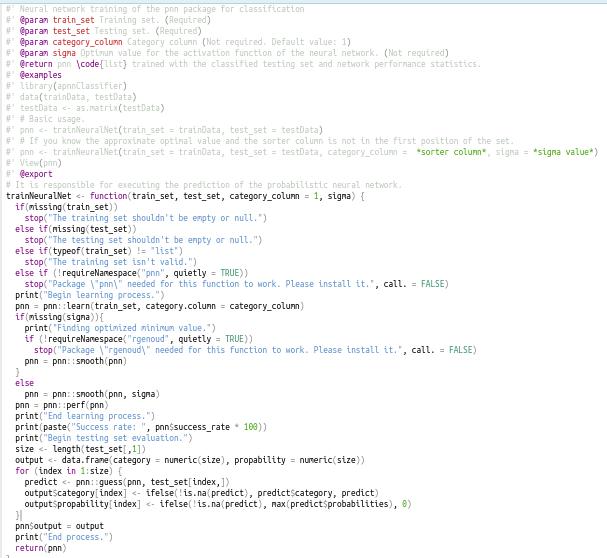
\includegraphics[scale=0.8]{codeTrainNeuralNet.png}
	\label{fig:codeTrainNeuralNet}
\end{figure}

\item \textbf{Función de evaluación de la red \textbf{(evaluate)}}, evalua la especificidad, efectividad y sensibilidad de la clasificación realizada por la red neuronal probabilística y depende del paquete de R \textbf{pROC} y \textbf{dPlyr}, la codificación de dicha función se muestra en la figura \ref{fig:codeEvaluate}.

\begin{figure}[h!]
	\caption{Codificación de la función de evaluación de la red neuronal probabilística.}
	\centering
	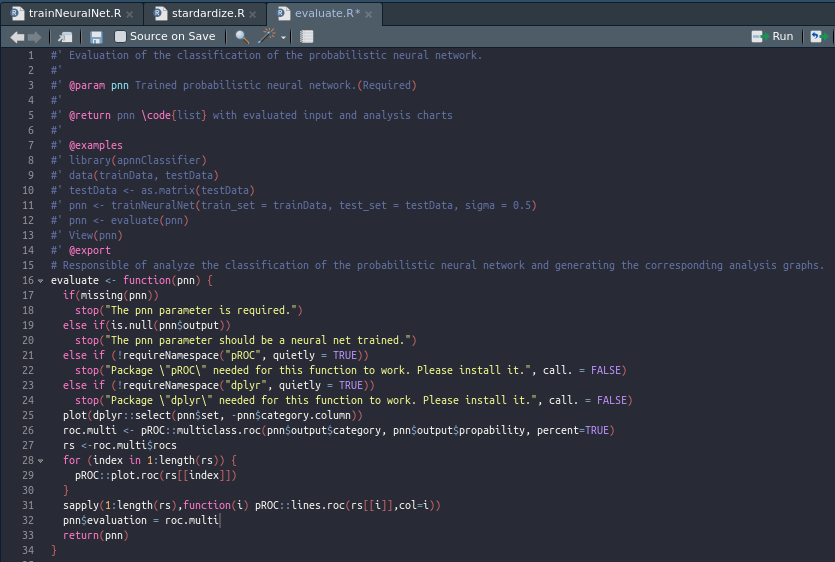
\includegraphics[scale=0.6]{codeEvaluate.png}
	\label{fig:codeEvaluate}
\end{figure}

\item \textbf{Función de estandarización de datos \textbf{(standardize)}}, se encarga de estandarizar los datos basado en dos tipos de estandarización para datos discretos o continuos, la codificación de dicha función se muestra en la figura \ref{fig:codeStandardize}.\\

\begin{figure}[h!]
	\caption{Codificación de la función de estandarización de datos.}
	\centering
	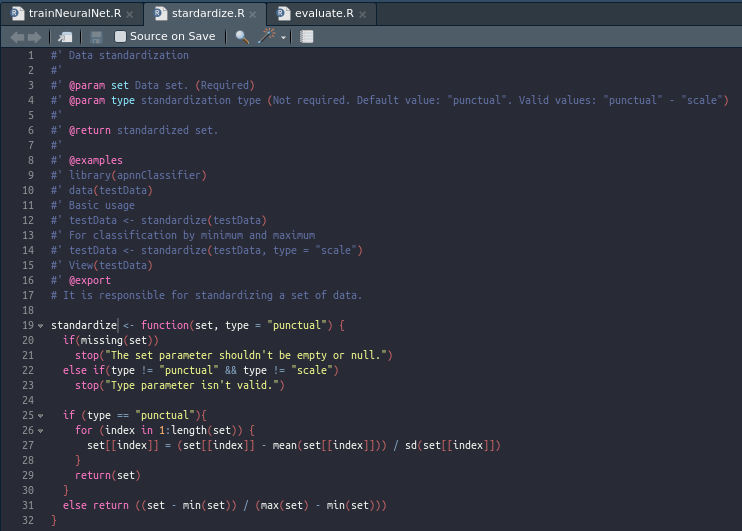
\includegraphics[scale=0.8]{codeStandardize.png}
	\label{fig:codeStandardize}
\end{figure}

\end{itemize}

\section{Chequeo del paquete, método de distribución y registro del método de envío.}

	Para realizar el chequeo del paquete se utilizaron las pruebas unitarias proporcionadas por los paquetes R \textit{RUnit} (Zenka, 2015) y \textit{testthat} (Wickham, 2017). Ver Figura \ref{fig:check}.\\

\begin{figure}[h!]
	\caption{Opción check para realizar el chequeo del paquete.}
	\centering
	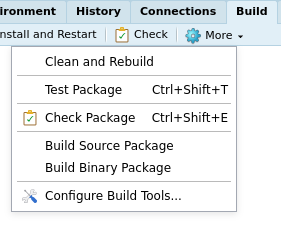
\includegraphics[scale=0.75]{check.png}
	\label{fig:check}
\end{figure}

	Para el método de distribución se utilizara \textit{tar.gz}, que es utilizado por defecto por RStudio. Ver figura \ref{fig:build}. \\
	

\begin{figure}[h!]
	\caption{Opción Build Source Package.}
	\centering
	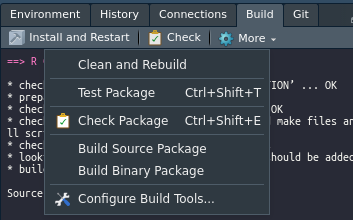
\includegraphics[scale=0.8]{build.png}
	\label{fig:build}
\end{figure}
	
	Como método de envío local se utilizará la plataforma de \textit{GitHub}.\\
	
\section{Pruebas funcionales del paquete}

	El objetivo de este trabajo investigativo consiste en realizar un clasificador de tubérculos de papa criolla para diferentes densidades de siembra y la solución se planteó desarrollando un paquete en R que empleando redes neuronales probabilísticas permitiera dicha clasificación. Para las pruebas funcionales del paquete se realizó la corrida de un algoritmo que permitiera a través del paquete clasificar tubérculos de papa con los datos recogidos en la investigación de Bernal, 2017. \\
	
	Las características que se tomaron para dicha prueba fueron el diámetro medio ponderado, el peso fresco y la cantidad de papas de un conjunto de 2840 datos de campo recogidos en la investigación de Bernal en 2017 (figura \ref{fig:input}). Dicho conjunto de datos fue dividido para la ejecución de las pruebas funcionales en un 75\% para el conjunto de entrenamiento y un 25\% para el conjunto de pruebas. Dicha segmentación se realizó de manera aleatoria por densidad de siembra para asegurar obtener resultados de valor.\\
	
\begin{figure}[h!]
	\caption{Conjunto de datos de entrenamiento.}
	\centering
	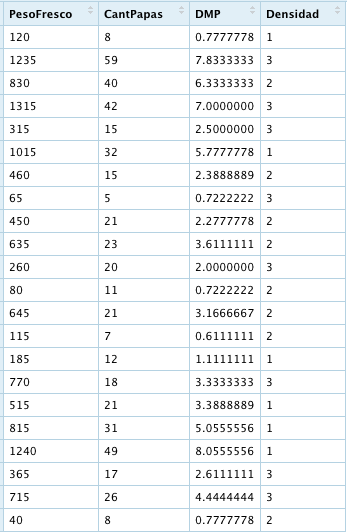
\includegraphics[scale=0.6]{input.png}
	\label{fig:input}
\end{figure}

La codificación de la anterior división, así como el uso de cada una de las funciones del paquete para permitir la clasificación de tubérculos de papa criolla (Solanum phureja) con mencionados conjuntos de datos como entradas se puede observar en la figura \ref{fig:packageuse}.\\

Los resultados obtenidos por el algoritmo se observan en las figuras \ref{fig:cloudpoints} y  \ref{fig:roc}. El concepto de las curvas ROC es contrastar la especificidad (fracción de verdaderos negativos) con la sensibilidad (fracción de verdaderos positivos). Una buena clasificación es caracterizada porque estos dos cálculos se comporten de manera inversamente proporcional, por lo que aunque las correlaciones sean altas entre las variables de entrada como se puede observar en el gráfico de nubes de puntos, no se obtiene una buena clasificación ya que para valores altos de sensibilidad se pueden observar valores altos de especificidad.\\

\begin{figure}[h!]
	\caption{Codificación del algoritmo de clasificación usando \textit{apnnClassifier}.}
	\centering
	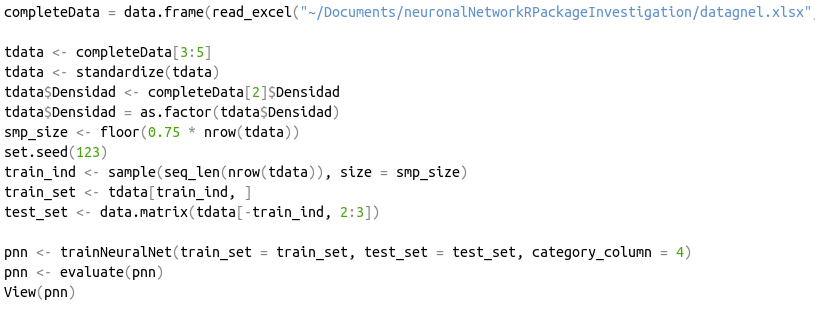
\includegraphics[scale=0.6]{packageuse.png}
	\label{fig:packageuse}
\end{figure}

\begin{figure}[h!]
	\caption{Gráfico de nubes de puntos.}
	\centering
	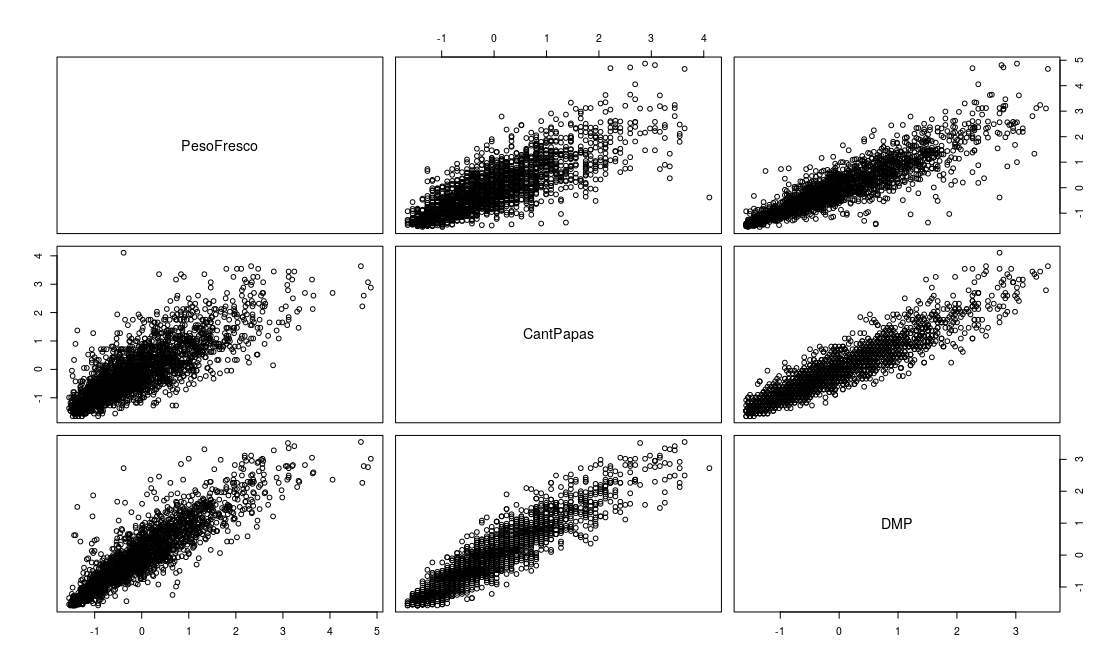
\includegraphics[scale=0.6]{cloudpoints.png}
	\label{fig:cloudpoints}
\end{figure}

\begin{figure}[h!]
	\caption{Gráfico de curva característica operativa de receptor.}
	\centering
	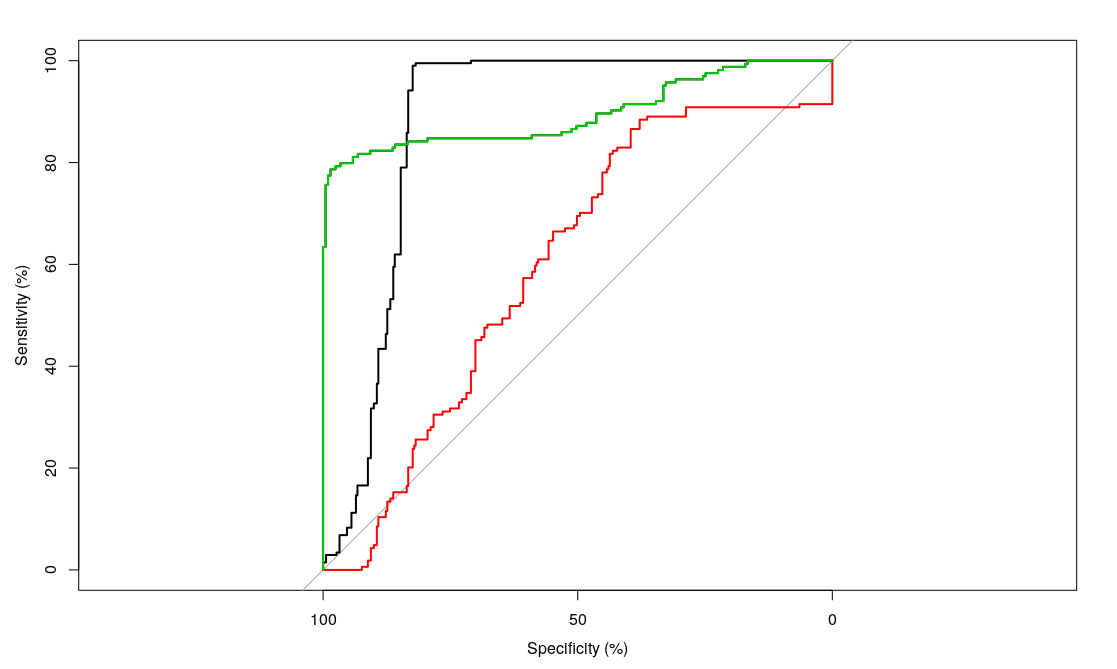
\includegraphics[scale=0.5]{roc.png}
	\label{fig:roc}
\end{figure}